\chapter[Why Carbon Builds So Many Structures]{Why Carbon Builds\protect\\ So Many Structures}

\begin{kaichang}
Volume I's final chapter left a mystery: how can the complex molecules of your skin, hair, muscles, rice, and eggs, assembled from hundreds or thousands of atoms, exist at all? We promised the answer through one special atom, carbon. Now Volume II begins, and it is time to solve the case.

Play a game like the one opening Volume I. Find four things nearby: a pencil, meaning its core rather than its wood; a sugar cube; a plastic bag; and the back of your own hand. All four share a chemical protagonist: carbon. Pencil cores are almost pure carbon; sugar's framework is carbon; plastic bags contain absurdly long carbon chains; and after subtracting your body's water, nearly half the remaining dry material is built from carbon.

Add a more dramatic comparison: pencil cores are black, soft, and readily shed particles, while diamond is transparent and the hardest natural substance. Yet both are \textbf{pure carbon}, with identical atoms, none added or missing.

Guess why the same atoms can build black and transparent, soft and hard, edible and combustible materials. Write down your answer and return to check it at the end.
\end{kaichang}

\section{One Atom, a Whole Zoo}

First, lay out the visible facts.

Carbon-containing substances are astonishingly numerous. More than two hundred million known substances have now been registered by chemists, and \textbf{the vast majority} contain carbon. All non-carbon ``inorganic substances'' together are only a small fraction. Hundreds of thousands of new carbon molecules are synthesized each year, and the list keeps growing wildly. Because these molecules were first extracted from organisms, chemists gave them the old name \textbf{organic compounds}. We will unpack that historical baggage later; for now, organic chemistry is essentially carbon chemistry.

Look at their range of personalities: methane is an easily ignited gas; gasoline is a water-insoluble liquid; sugar is a water-soluble solid; alcohol evaporates rapidly and burns the throat; rubber stretches and springs back; nylon forms fibers stronger than steel wire. Diamond and graphite are extremes of the same element. Carbon anchors every framework, yet hardly any two behave alike.

Recall the book's five recurring questions: (1) What is it made of? (2) How are its parts connected and arranged? (3) What energy and probability rules determine whether it changes? (4) How fast does change occur, and how is it controlled? (5) How is it maintained, copied, regulated, and selected in life? Volume I mainly answered (1) and parts of (3) and (4). This chapter and all of Part V center on question (2): \textbf{connection and arrangement}. Those alone can explain carbon's million-strong army.

\section{Carbon's Four Hands}

Zoom down to atoms. Carbon has six nuclear protons and six electrons arranged by Chapter 9's floor rules: two on the first floor, four on the second. Those four outermost electrons are the key.

Four is awkward. Recall Chapter 18: sodium's one outer electron is cheap to lose, so it readily becomes an ion; chlorine's seven need only one more to fill the shell, so it grabs electrons. Carbon must pay four increasingly expensive ionization fees to lose four, or force four negative charges into one atom to gain four, creating enormous repulsion. Both routes are too costly, so it chooses Chapter 19's third route, \textbf{covalent bonding}: neither give nor grab, but share electron pairs with neighbors. Four outer electrons allow participation in four shared pairs:

\textbf{A carbon atom can extend at most four ``hands,'' forming four covalent bonds.}

Four hands are not unique to carbon: silicon has four, nitrogen three, oxygen two. Carbon's special skill is that \textbf{holding hands with itself is particularly secure}. A carbon--carbon single bond has energy around \ud{350}{kJ/mol}. Chapter 17 defined bond energy as the average cost of breaking a bond. This is a subtle balance: strong enough to keep chains intact at body and room temperatures, but not so strong that rebuilding requires unaffordable demolition costs. Compare neighboring elements: oxygen--oxygen and nitrogen--nitrogen single bonds have about half carbon--carbon's strength because opposing lone pairs repel, making chains easier to break. Silicon--silicon bonds are too long and weak; silicon chains soon fall apart in air. Across Group 14's first through fifth floors, only carbon joins itself into long chains so well and reliably.

Carbon's world therefore starts this way: carbon atoms hold hands to make chains, each reaching at most four partners, with unused hands grasping hydrogen, oxygen, or nitrogen attachments. Chains can lengthen, branch, or bite their own tails into rings. The next section explores these variations.

\section{Chains, Rings, Branches: Exploding Possibilities}

Start with the simplest rules: every carbon has four hands; unused hands hold hydrogen. Two carbons make ethane, \chem{CH_3-CH_3}; three make propane, \chem{CH_3-CH_2-CH_3}. Each has only one connection pattern. Four carbons introduce alternatives: all four can line up, or three form a chain with the fourth attached to its middle carbon, like a tree branch. Five carbons have three patterns, six have five, and so on.

This is carbon's first structural secret: \textbf{the same numbers of atoms can connect differently}. The number of patterns grows ferociously with carbon count.

\begin{qiaoliang}
For molecules containing only carbon and hydrogen, with only carbon--carbon single bonds, the alkanes of Chapter 39, let the carbon count be $n$. How many different connection patterns exist? Mathematicians have thoroughly solved this counting problem. The first few values are:

\begin{center}
\begin{tabular}{cccccccc}
\toprule
Carbons $n$ & 4 & 5 & 6 & 8 & 10 & 15 & 20 \\
\midrule
Patterns & 2 & 3 & 5 & 18 & 75 & 4347 & 366319 \\
\bottomrule
\end{tabular}
\end{center}

Look at the trend: each added carbon roughly more than doubles the possibilities, an \textbf{exponential} increase. The thirty-carbon alkane \chem{C_{30}H_{62}} theoretically has about $4.1\times 10^{9}$ connection patterns. Estimate the scale: drawing one per second, with about $3.2\times 10^{7}$ seconds per year, would take $4.1\times 10^{9}\div 3.2\times 10^{7}\approx 130$ years. That permits only thirty carbons and single bonds! One protein in your body contains thousands of carbons. Carbon does not merely build many structures: it builds \textbf{more than the entire universe could ever make}.
\end{qiaoliang}

Besides branching, chains can join head to tail into rings. Six-membered rings formed from six carbons are especially common: glucose has one, and gasoline and medicines are full of them. Rings can stand alone, fuse alongside one another, or bridge together, interlinking like bicycle-chain links. Chains, branches, and rings freely combine into the entire grammar of carbon frameworks. Only one rule applies: every carbon always has four hands.

\section{Three Dimensions: Tetrahedra and Joints}

So far we have drawn molecules on paper, as though carbon chains were flat. They are not. Carbon is three-dimensional.

Recall Chapter 20's electron-pair repulsion model: four bonds mean four mutually repelling electron pairs, with lower energy when farther apart. In a plane, the best separation is a cross with $90^{\circ}$ angles. In three dimensions, however, bonds can point toward the corners of a \textbf{regular tetrahedron}, each angle about $109.5^{\circ}$, the lowest-energy arrangement. A carbon with four neighbors is therefore not cross-shaped but tetrahedral: carbon at the center, four hands toward four corners.

This detail brings two far-reaching joint rules:

\begin{itemize}[itemsep=2pt]
\item \textbf{Single bonds are rotating joints}. When two carbons share one electron pair, their bond resembles a round axle whose ends can rotate relative to each other. A chain in liquid constantly twists, folds, and swings like a snake changing posture. These postures are not different molecules: rotation brings them back.
\item \textbf{Double bonds are locked joints}. With two shared electron pairs, the double bond of Chapter 19, the second pair is like welding the round axle into a square one. The ends \textbf{cannot} rotate freely: turning requires first breaking the second bond, at substantial energy cost. Once atoms at the ends are fixed on the same or opposite sides, they are locked there.
\end{itemize}

The difference between rotating and locked sounds small, but later you will see how much it changes: whether plastic draws into fibers (Chapter 43), whether fat is oil or wax (Chapter 40), and even whether cell membranes are soft or stiff all answer to these rules.

\section{Four Ways to Draw Carbon Frameworks}

Invisible molecules must be put on paper. Over centuries, chemists developed four increasingly detailed drawing languages. Use the straight-chain four-carbon molecule butane:

\begin{itemize}[itemsep=2pt]
\item \textbf{Molecular formula}: \chem{C_4H_{10}}. An ingredient list, counting carbon and hydrogen without connections. Minimal information, enough to address an envelope.
\item \textbf{Condensed structural formula}: \chem{CH_3-CH_2-CH_2-CH_3}. Each carbon's hydrogens are shown, with dashes marking carbon connections. Connectivity is clear, but still flat.
\item \textbf{Skeletal formula}, or bond-line formula: a quicker sketch, drawing only carbon--carbon bonds as a zigzag. \textbf{Every endpoint and corner is a carbon}. Carbon symbols and their hydrogens are omitted: every carbon must have four hands, so fill missing ones with hydrogen. Organic chemists use this language daily, and this book increasingly will too.
\item \textbf{Ball-and-stick model}: balls represent atoms, sticks covalent bonds, constructing tetrahedra and angles in three dimensions. Most informative, but most space-consuming.
\end{itemize}

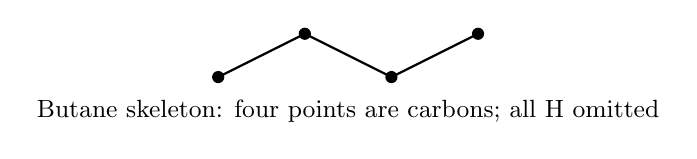
\begin{tikzpicture}[scale=1.1]
\draw[thick] (0,0) -- (1,0.5) -- (2,0) -- (3,0.5);
\fill (0,0) circle (2pt);
\fill (1,0.5) circle (2pt);
\fill (2,0) circle (2pt);
\fill (3,0.5) circle (2pt);
\node[below] at (1.5,-0.15) {\small Butane skeleton: four points are carbons; all H omitted};
\end{tikzpicture}

All four, remember, are \textbf{human conventions for representation}. Real molecules contain no sticks, nor are electrons two beads sitting on them, as Chapter 19 stressed. Omitted carbons and hydrogens still exist; readers are expected to supply them. The simpler the drawing, the more information you must reconstruct mentally: a basic skill in reading organic structures.

\section{How Chemists Knew Carbon Was Tetrahedral}

Molecules are tiny, you say: who ever saw a tetrahedron? Good question. This is the chapter's most worthwhile detective story.

\begin{zhengju}
By the mid-nineteenth century, chemists knew carbon was tetravalent, but not which way its four bonds pointed. In 1874, the twenty-two-year-old Dutchman van 't Hoff and twenty-seven-year-old Frenchman Le Bel independently published almost simultaneously the same bold claim: \textbf{carbon's four bonds point to a tetrahedron's corners}.

Their elegant reasoning needed no view of molecules, only \textbf{counting isomers}. Start with facts: replacing one hydrogen of methane, \chem{CH_4}, with chlorine yields only one \chem{CH_3Cl}. Replacing two yields \chem{CH_2Cl_2}, and decades of synthesis, fractional distillation, and melting- and boiling-point measurement found only \textbf{one} kind. Test a hypothesis: if four bonds lay in one plane, say at square corners, adjacent and opposite chlorine pairs should give \textbf{two} different \chem{CH_2Cl_2} molecules, with different properties and separable identities. Experiments stubbornly gave only one. Evidence cornered the planar hypothesis. In a tetrahedron, every pair of vertices is adjacent, so dichloromethane naturally has one form, matching observation.

Were alternatives seriously excluded? Yes. Perhaps nobody had yet made the second \chem{CH_2Cl_2}? Chemists tried many synthetic routes for decades without finding it. Perhaps both existed but interconverted too fast to separate? This sophisticated objection forced stronger evidence. The tetrahedral model predicted that carbon attached to four \textbf{different} groups should produce left- and right-handed molecules: nearly identical physical properties, nonsuperimposable mirror images, and no interconversion by rotation. Such pairs were indeed found. As early as 1848, Pasteur had used tweezers and a microscope to sort two tartaric-acid crystal forms, without anyone then explaining why. Prominent chemists publicly mocked van 't Hoff's booklet as the fantasy of a dreamer riding Pegasus. But early in the twentieth century, the Braggs used X-ray diffraction to measure diamond's four neighbors around each carbon at tetrahedral vertices, grounding the supposed fantasy in fact. Van 't Hoff later received the first Nobel Prize in Chemistry.

The method parallels Mendeleev's: begin with countable numbers, leave wrong shape hypotheses nowhere to hide, and stake the model on falsifiable predictions such as mirror-image pairs. You need not see molecules to know their shapes, provided your counts are solid enough.
\end{zhengju}

\section{Same Atoms, Different Molecules: Isomers}

Now name the alternatives encountered repeatedly. Molecules with the same molecular formula, an identical ingredient list, but different structures are \textbf{isomers}. They are not different spellings of one substance, but genuinely different substances, with different boiling points, smells, and toxicities, separable into their own bottles. By the level of difference, three families emerge:

\textbf{First: constitutional isomers, with different connections.} The four carbons of \chem{C_4H_{10}} can form straight or branched chains, giving n-butane and isobutane. Their boiling points are about $-0.5\,^{\circ}\mathrm{C}$ and $-12\,^{\circ}\mathrm{C}$ respectively; lighters and aerosol cans often contain mixtures. Connectivity differences also include attaching the same group at different chain positions, or dividing the same formula into different kinds of groups. Both involve attachments themselves, discussed under functional groups in Chapter 37.

\textbf{Second: cis--trans isomers, with different positions beside a locked joint.} Double bonds cannot rotate freely, so groups at their ends on the same side, cis, or opposite sides, trans, make different molecules. For two double-bonded carbons each bearing a methyl group, the cis form boils around $4\,^{\circ}\mathrm{C}$ and trans around $1\,^{\circ}\mathrm{C}$: a small but separable difference. Life amplifies it. Most double bonds in natural plant oils are cis, bending molecules into elbows that pack poorly, so they remain liquid at room temperature. Some processing turns double bonds trans, straightening molecules, improving packing, and raising melting points. This is the origin of ingredient-label trans fatty acids, whose excessive intake is associated with cardiovascular risk. Chapter 49's lipids will examine dose and evidence.

\textbf{Third: enantiomers, nonsuperimposable mirror images.} Carbon bearing four different groups resembles a hand: left- and right-handed molecules share formula and connectivity but are different substances, the pair van 't Hoff predicted. Their behavior can differ enormously because enzymes and receptors are themselves chiral, recognizing one hand but not the other. The story is too long and important for here: Chapter 42 covers it. For now, remember that \textbf{mirror images are not always equivalent in the molecular world}.

A molecule can layer several kinds of isomerism: different connectivity compared with another molecule, double-bond positioning within its own framework, and mirror-image forms. As carbon frameworks grow, these same-formula, different-structure branches spread exponentially, recruiting organic chemistry's million-strong army.

\section{Where Are the Models' Boundaries?}

As always, a model has both instructions and failure zones.

First, \textbf{every drawing is a representation}. Ball-and-stick models make hard spheres and rods to aid spatial reasoning, not to depict real atoms and bonds. Skeletal formulas omit almost everything. Reason with them, but do not mistake them for photographs.

Second, \textbf{free single-bond rotation is approximate}. Rotation crosses a small energy barrier and becomes hesitant at low temperature. A carbon incorporated into a ring has its rotation locked, making ring geometry important. Three- and four-carbon rings are especially strained: a tetrahedron wants $109.5^{\circ}$, but cyclopropane forces angles to $60^{\circ}$. Bent bonds raise energy, and this ring strain makes small rings particularly prone to opening reactions. Our freedom to form rings requires qualifications for three- and four-membered ones.

Third, \textbf{we deliberately undercounted isomers}. The table counts connectivity only; include cis--trans and mirror-image forms, and numbers grow much larger. Conversely, it can overcount: some drawable structures are extremely unstable because atoms collide through steric hindrance, and may never be made. The model lists possibilities; nature and laboratories perform a second selection.

Fourth, \textbf{one carbon framework resists this chapter's drawings}: benzene. Its six carbons have no true distinction between single and double bonds; electrons are distributed around the whole ring. Forcing alternating single and double bonds into a picture misses its unusual stability. Chapter 41 focuses on this; here, simply note the warning sign.

\begin{wuqu}
``Organic means natural and made by life; natural means safe and healthy, while synthetic means harmful.'' Both claims are wrong, in ways worth unpacking.

First, organic's historical baggage: early nineteenth-century chemists believed only a vital force in organisms could make organic substances, beyond laboratory reach. In 1828, the German chemist Wöhler heated the inorganic salt ammonium cyanate and unexpectedly obtained urea, a genuine organic substance in mammalian urine. No vital force inhabited the beaker, yet urea formed. The wall equating organic with life-made collapsed. Today organic chemistry has only a technical definition, carbon-framework chemistry, independent of origin. Laboratories can synthesize insulin; bacteria can naturally make botulinum toxin.

Now natural safety: amatoxins in poisonous mushrooms, tetrodotoxin in pufferfish, and aflatoxin on moldy peanuts are entirely natural organic molecules and all highly toxic. Meanwhile aspirin, insulin, and vaccine adjuvants, made synthetically or semisynthetically, have saved countless lives. Judge safety by structure, dose, exposure route, and evidence, Chapter 35's detective attitude, not origin. Incidentally, skincare advertising's chemical-free claim is semantically empty: water is a chemical, and you yourself are a chemical factory.
\end{wuqu}

\begin{shiyan}
\textbf{Build Carbon Frameworks by Hand} (safe household materials).

Materials: modeling clay in two or three colors, or peeled cooked quail eggs, grapes, or marshmallows; a box of toothpicks; a ruler.

Step one: build methane. Make one large carbon ball and four small hydrogen balls. Insert four toothpicks into carbon, each ending in a hydrogen. Adjust them so \textbf{every pair of angles is as equal as possible}. In a plane, some angle remains too small; only lifting one and pointing all four into space equalizes them. Measure distances between neighboring toothpick tips: in a tetrahedron all six distances should be roughly equal. Your hands have encountered $109.5^{\circ}$.

Step two: build two butanes. Take four medium carbon balls and connect them with three toothpicks in a straight chain. Reassemble them into a three-carbon chain with the fourth on the middle carbon. Did the number of balls or toothpicks change? No, but the shapes cannot match. These are \chem{C_4H_{10}}'s two isomers.

Step three: join a six-carbon chain head to tail into a ring. Try to keep toothpick angles near tetrahedral: the ring naturally rises into a little chair rather than lying flat.

Step four: build a locked joint. Insert \textbf{two} parallel toothpicks between two balls for a double bond and attach small balls at both ends. Try twisting as with a single bond: toothpicks jam, preventing rotation or breaking. Your hands now understand why double bonds cannot rotate freely.

What to observe: step one's uneven planar but even spatial arrangement; step two's equal ball count but mismatched structures; step four's jamming toothpicks.

Safety: toothpicks are sharp. Keep them away from eyes and faces, and never put them in your mouth. If using grapes or marshmallows, wash your hands afterward and \textbf{do not eat} food touched by modeling clay and toothpicks.
\end{shiyan}

\section{Back to the Four Objects}

Now check your guesses. Why do pencil cores and diamond differ so much? Chapter 24 already solved this: each carbon in diamond holds four neighbors, weaving a three-dimensional network in all directions. Moving any carbon requires breaking several bonds at once, producing exceptional hardness. In graphite, each carbon extends only three hands to form flat hexagonal fishing nets. No true chemical bonds join layers; weak intermolecular forces from Chapter 22 stack them, allowing easy sliding. Writing means layers slide off graphite and remain on paper. Identical atoms with \textbf{different connections} make one a master glass scratcher and the other a writing tool.

What about sugar and plastic? Their carbon frameworks carry different attachments. Sugar bristles with water-loving claws and dissolves; polyethylene (Chapter 43) is a plain carbon chain bearing thousands of hydrogens, long enough to tangle into atomic spaghetti, making it flexible and waterproof. The proteins, fats, and DNA in the back of your hand also obey the four-hand carbon rule, but their attachment types and arrangements have another level of intricacy. What those attachments are, and how they determine personality, comes next.

Did you guess it? This is the full power of recurring question (2): identical composition, different \textbf{connections and arrangements}, completely different worlds. Volume I taught what things are made of, whether they change, and how fast. From here, how they connect, arrange, and point takes center stage.

\section{Framework Ready: What about Its Interfaces?}

This chapter considered only frameworks: chain length, branches, rings, and locked or rotating joints. A framework alone is mute; pure carbon chains do little beyond burn (Chapter 39) or tangle into plastic (Chapter 43). What makes an organic molecule sour, fragrant, intoxicating, or medicinal is its specific interfaces: attach oxygen here, and it becomes alcohol; add another oxygen, and it becomes vinegar; place nitrogen elsewhere, and it might become a drug.

These interfaces share a name: \textbf{functional groups}. Next chapter introduces their family of standard parts. You will discover that millions of organic molecular personalities depend on just a dozen or so interfaces.

\begin{tiaozhan}
\textbf{Challenge: can you count all five isomers of \chem{C_6H_{14}} without duplication or omission?} Skipping this section does not break the main thread.

Random drawing guarantees repeats and omissions; use systematic search. Start with the longest main chain and shorten it step by step:

First, a six-carbon main chain gives one straight-chain structure.

Second, a five-carbon main chain leaves one branch carbon, attachable only at position 2 or 3. Position 1 extends the chain, and position 4 duplicates position 2 by symmetry. Two structures.

Third, a four-carbon main chain leaves two carbons, either two methyl groups or one ethyl. An ethyl branch lengthens the effective main chain and repeats earlier structures, so only two methyls remain: positions (2,2) or (2,3), giving two structures.

Fourth, a three-carbon main chain cannot accommodate three branch carbons without duplication: zero structures.

Total $1+2+2=5$, matching the table. Shorten the main chain, move branches, check repeats: an intuitive version of computational molecule-enumeration algorithms. Try \chem{C_7H_{16}}, with nine as the answer, and appreciate why humans wrote programs to count them.
\end{tiaozhan}

\section*{Try It Yourself}

\begin{sikaoti}
\item Without consulting references, write condensed structural formulas for all three \chem{C_5H_{12}} isomers and draw each skeletal formula. Does every carbon have exactly four hands?
\item A student draws two supposedly different butanes: a straight chain, and the same chain bent in the middle. Are they isomers? Explain using the rotating-single-bond rule.
\item Ethene, \chem{C_2H_4}, has a carbon--carbon double bond. Replace one of each carbon's two hydrogens with chlorine. How many different molecules result? Why is the number different if you make the same substitutions in single-bonded ethane, \chem{C_2H_6}? Draw particle arrangements and explain.
\item Diamond and graphite are pure carbon. Using connections and arrangements, explain to a friend without chemistry background why diamond scratches glass while pencil cores shed powder when writing. No circular arguments saying hardness differs because hardness differs.
\item What do a skeletal formula's endpoints and corners represent? Draw a skeletal formula for this molecule: \chem{CH_3-CH(CH_3)-CH_2-CH_3}. Then count its carbon and hydrogen atoms.
\item Van 't Hoff had no X-rays yet asserted tetrahedral carbon bonds. What kind of evidence did he use? Imitate his counting argument: if three carbon bonds lay on paper and one stood perpendicular, making a pyramidal arrangement, how many \chem{CH_2Cl_2} forms should exist? What observation rules this model out?
\end{sikaoti}
